\chapter{Evaluation}
\label{evaluation}
In previous chapters detailed working of the planning algorithm has been discussed, this chapter discusses the evaluation criteria and results in detail. Various concepts discussed previously will be examined here through a series of experiments reflecting real-life driving scenarios. This chapter is organised as follows: Section \ref{experiments} discusses the systematic evaluation of the planner by exposing it to various situations equivalent to on-road driving conditions. The next section \ref{criteria_based_eval} discusses a criteria-based assessment for the planner by examining factors such as feasibility, optimality, completeness, run-time etc.

\section{Experiments}\label{experiments}
Due to time and resource constraint, most of the experiments to evaluate the planner are performed on the simulator. The test cases involve finding a collision-free path with obstruction in driving lane, avoiding slow moving traffic, merging into ongoing traffic, lane changes etc. The following subsections detail further on each experiment. 

\subsection{Lane blocked}
In driving scenario  \ref{lane_blocked_1}, driving lane is blocked by a static obstacle and a slow-moving obstacle is in the next lane, here ego vehicle drives slowly till it finds enough room in the next lane, once the obstacle is avoided the robot continues to shift into the intended lane and drives with increasing speed. 

\begin{figure}[h]
    \centering
    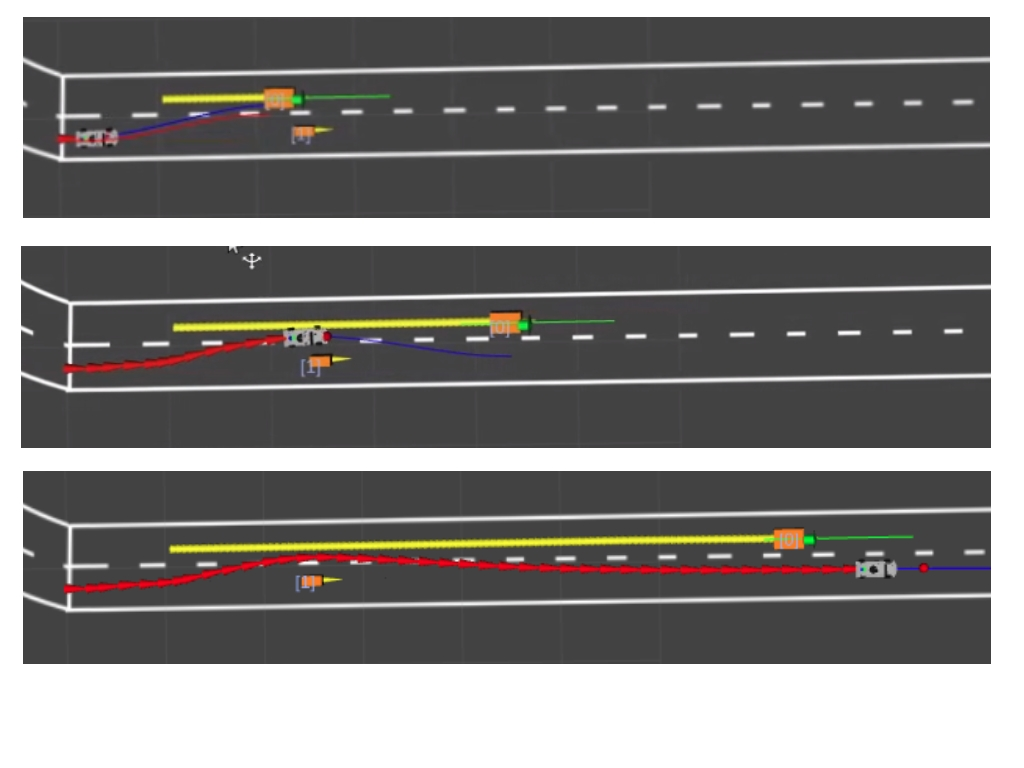
\includegraphics[width=0.7\textwidth]{Images/evaluation/2_lane_blocked.jpg}
    \caption{Driving Lane is blocked by a static obstacle with an obstacle moving in next lane. The ego vehicle avoids the static obstacle by driving into next lane and comes back to intended lane once it is free}
    \label{lane_blocked_1}
\end{figure}

\subsection{Slow Moving Traffic}
In situation one presented in Figure \ref{slow_moving_1} ego vehicle starts changing into left lane once a slow-moving obstacle is encountered, once the obstacle is passed it starts driving into right lane again. In situation two presented in Figure \ref{slow_moving_2} there are two slow-moving obstacles ahead, once the ego vehicle overtakes the initial obstacle it shifts to the first lane as intended but it encounters the second slow-moving obstacle and shifts to left lane again. This behaviour is caused because of locally optimal cost functions driving the ego vehicle into the intended lane without knowledge of long-term planning information. A behavioural layer with longer scenario analysis horizon will result in better path selection.
\begin{figure}[h]
    \centering
    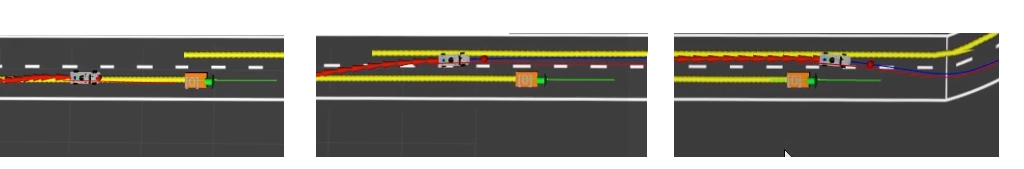
\includegraphics[width=0.8\textwidth]{Images/evaluation/slow_moving1.jpg}
    \caption{Slow Moving Traffic Situation 1}
    \label{slow_moving_1}
\end{figure}

\begin{figure}[h]
    \centering
    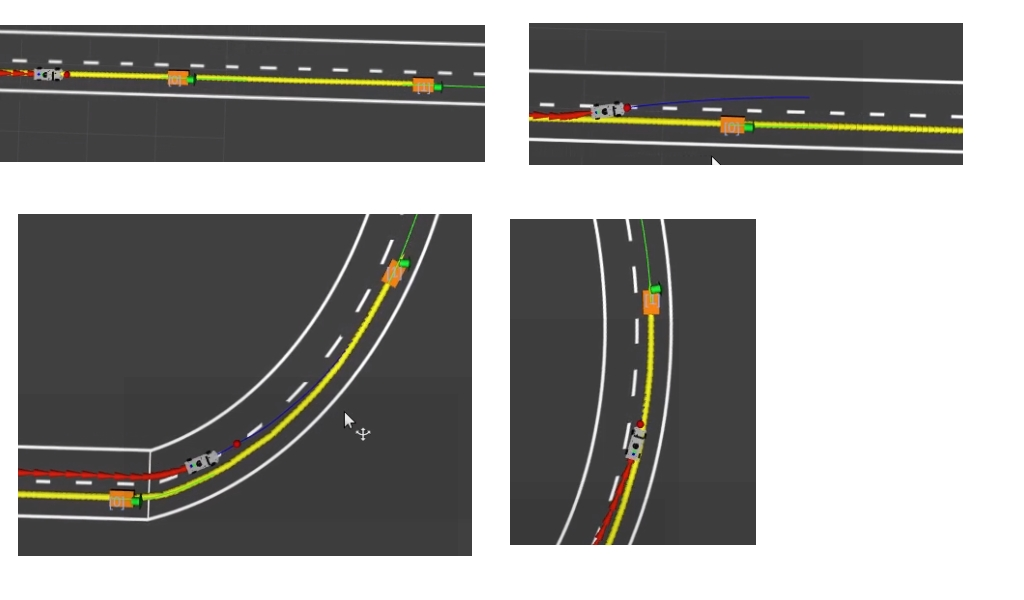
\includegraphics[width=0.8\textwidth]{Images/evaluation/slow_moving2.jpg}
    \caption{Slow Moving Traffic Situation 2}
    \label{slow_moving_2}
\end{figure}

\subsection{Merging into traffic}

In the scenario presented in Figure \ref{merging1}, lane changing is requested to merge into the traffic in the left lane. Here ego vehicle speed is $1ms^{-1}$ and obstacle speed is $0.6m^{-1}$. Initially, lane change does not occur as cost functions are tuned to maintain speed over maintaining required lane. As the vehicle enters the curve, target driving speed is reduced, and the vehicle merges into the traffic in the left lane. Depending on which portion of the lane the ego vehicle is in, i.e., near intersections or exits target lane should have higher priority over maintaining speed and during rest of the regions target speed should be of higher priority to reach a destination quickly. Cost functions implemented in this thesis provide flexibility in tuning behaviour of the ego vehicle. 

\begin{figure}[h]
    \centering
    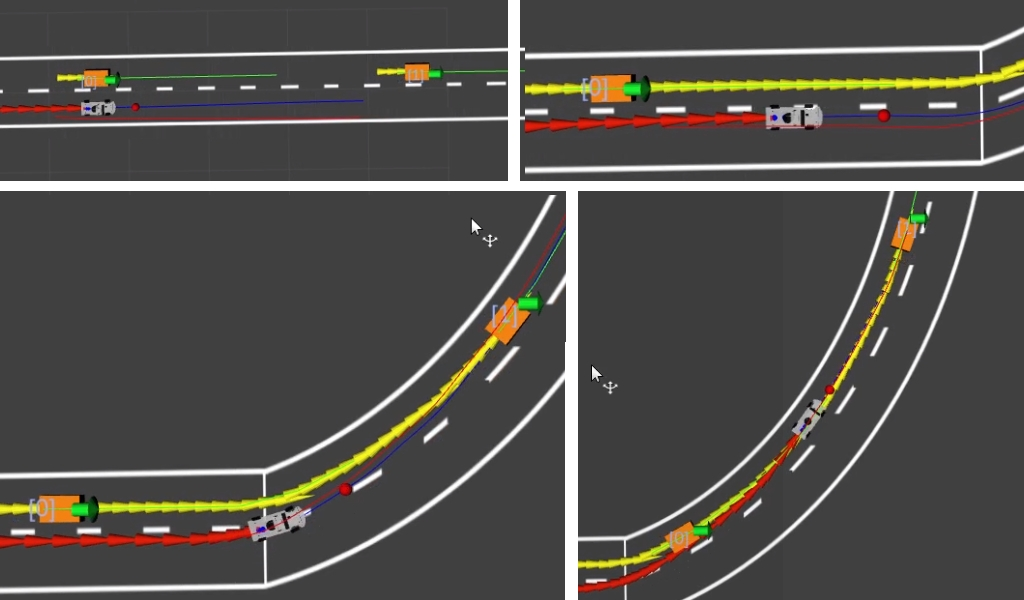
\includegraphics[width=0.8\textwidth]{Images/evaluation/merging1.jpg}
    \caption{Merging into Traffic}
    \label{merging1}
\end{figure}

\subsection{Merging into next lane with opposite traffic}

In the scenario presented in Figure \ref{series_obstacles} driving lane is blocked by a series of obstacles and the left lane is occupied by a moving obstacle. Ego vehicle starts slowly in the driving lane and waits till the obstacle is passed in the left lane and starts driving forward. 
\begin{figure}[h]
    \centering
    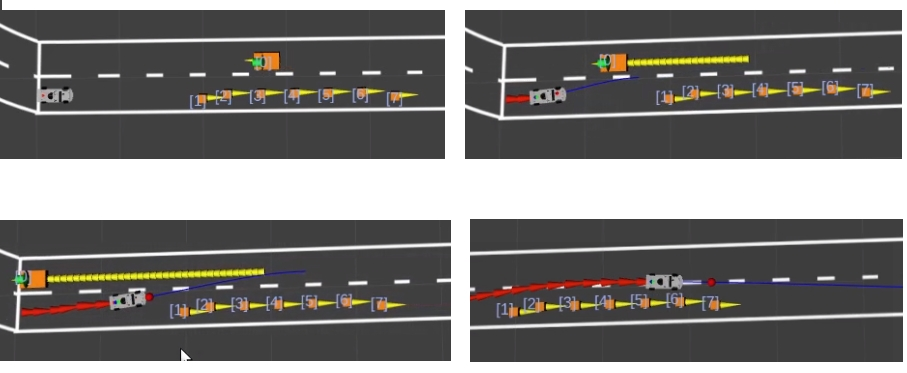
\includegraphics[width=0.8\textwidth]{Images/evaluation/series_lane_blocked1.jpg}
    \caption{Lane blocked by series of static obstacles and vehicle in next lane driving opposite}
    \label{series_obstacles}
\end{figure}

This situation may lead to ego vehicle getting stuck in the middle of the road. If driving speed of ego vehicle is low, temporal horizon limits ego vehicles lookahead distance into future. If a fast-moving obstacle in left lane not visible in 5 seconds of temporal horizon then the ego vehicle starts lane change. If an obstacle is detected after the start of lane change manoeuvre, the ego vehicle aborts if there is time to abort and if not the ego vehicle will stop in the middle of the lane due to no path ahead, if the obstacle proceeds without stopping for the ego vehicle. It can be avoided by a behavioural layer with longer spatial scenario analysis horizon. As the planner discussed in this thesis is not created for controlling the vehicle to drive backwards, a different planner equivalent to off-road planner must be used to clear the way.  


\subsection{Road Blocked or Pedestrian Ahead}

In the scenario presented in Figure \ref{road_blocked}, the road is blocked by a series of static obstacles, the vehicle enters the empty left lane, slows down and finally stops when it cannot find route ahead. 

\begin{figure}[h]
    \centering
    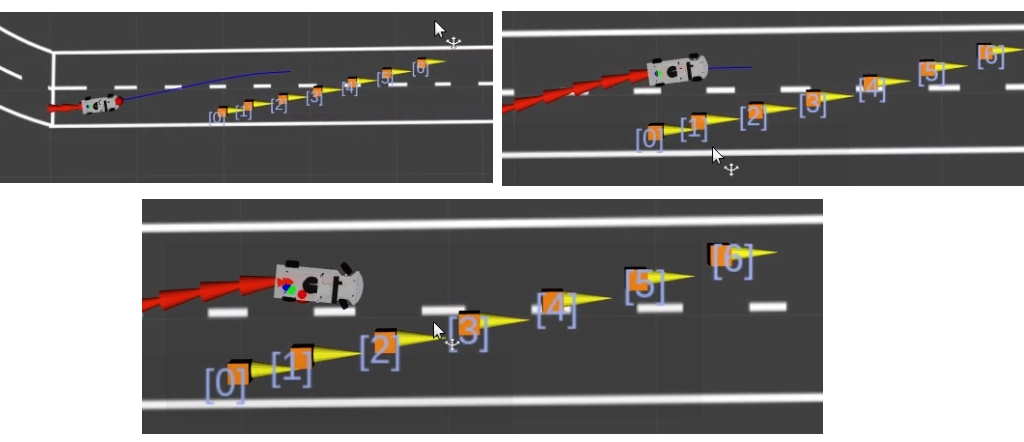
\includegraphics[width=1.0\textwidth]{Images/evaluation/road_blocked1.jpg}
    \caption{Road Blocked by series of obstacles}
    \label{road_blocked}
\end{figure}

A pedestrian on the road is considered similar to a road blocking, in this case as shown in Figure \ref{pedestrian_ahead} the ego vehicle initially drives at full speed, then the vehicle slows down(shorter blue line representing a slower speed), and the robot finally comes to a halt few meters ahead of the pedestrian. Buffer distance is a tunable parameter and currently at the maximum value for safety. 

\begin{figure}[h]
    \centering
    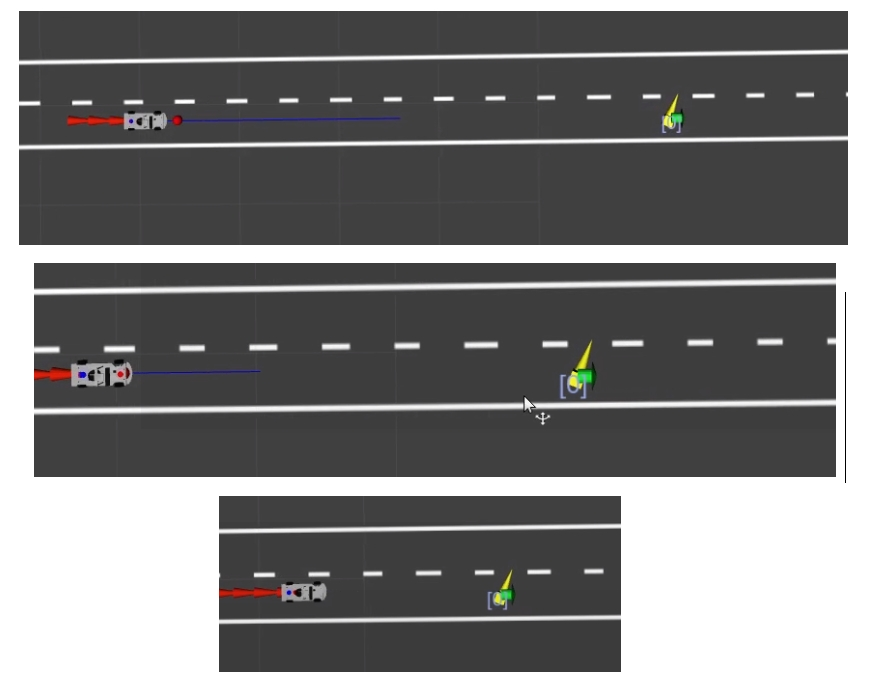
\includegraphics[width=0.8\textwidth]{Images/evaluation/pedestrian_ahead.jpg}
    \caption{Pedestrian Ahead on Road}
    \label{pedestrian_ahead}
\end{figure}

\subsection{Dynamic Obstacles - other vehicles}
The main objective of the planner is to adjust to the sudden changes in the environment caused by the dynamic obstacles in surroundings, here two sub-scenarios are described where the ego vehicle has to react to unexpected breaking of vehicles ahead. 

In scenario presented in Figure \ref{dynamic_1}, there are two situations. In situation one the car aborts a lane change when the slow-moving dynamic obstacle in the left lane is detected, then once the dynamic obstacle is passed the vehicle shifts to the left lane to avoid the stopped dynamic obstacle in driving lane. This situation is similar when a vehicle ahead stops to drop off a passenger or waiting for a parking spot. In situation two, the car doesn't choose lane change initially and slows down till it finds enough room in the left lane to drive ahead of the stopped dynamic obstacle. 

\begin{figure}[h]
    \centering
    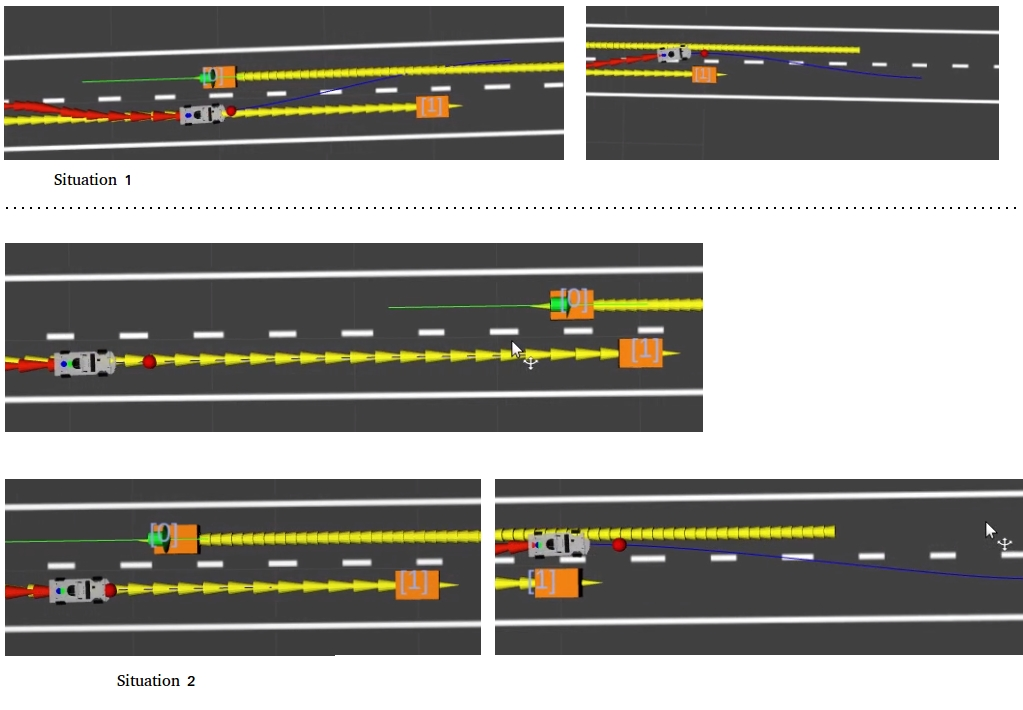
\includegraphics[width=0.8\textwidth]{Images/evaluation/dynamic_ahead_breaking1.jpg}
    \caption{Dynamic Obstacle Ahead stops in middle of road}
    \label{dynamic_1}
\end{figure}

In the scenario presented in Figure \ref{dynamic_2} there are two situations with different thresholds for safety, in situation one a safe 2s+ distance to obstacles ahead is chosen, here the ego vehicle stays far away from the vehicles ahead and when it stops it stops relatively farther from the vehicles ahead. In situation 2, the threshold has been adjusted to 0.5s leading to the aggressive behaviour of ego vehicle. The ego vehicle drives closer to the obstacles ahead, and when the dynamic obstacles ahead stop suddenly, the distance between the ego vehicle and the obstacles ahead is very narrow.   
\begin{figure}[h]
    \centering
    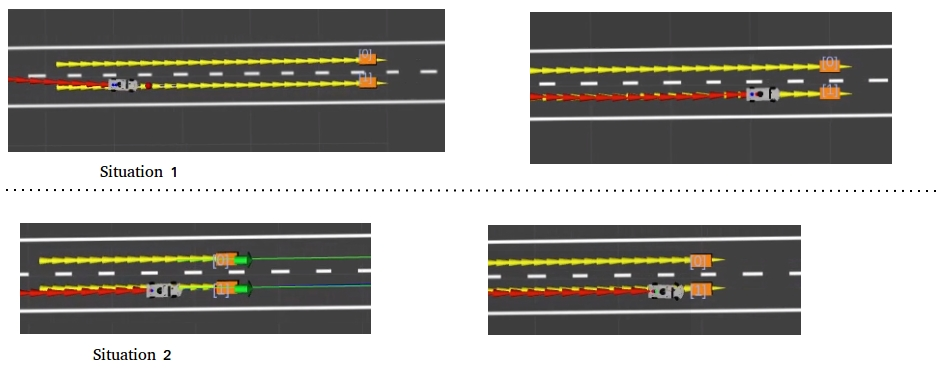
\includegraphics[width=0.8\textwidth]{Images/evaluation/dynamic_ahead_breaking2.jpg}
    \caption{Two Dynamic Obstacles ahead stop suddenly}
    \label{dynamic_2}
\end{figure}

%\subsection{Avoiding Static Obstacles}
%\subsection{Avoiding Dynamic Obstacles}
%\subsection{Avoiding Pedestrians}
%\subsection{Lane Changing}
%\subsection{Series of Static Obstacles}
%\subsection{Road Blockades}
%\subsection{Intersection}
%\subsection{Oncoming traffic}
%\subsection{Dynamic Obstacle breaking suddenly}
%\subsection{Merging into traffic to avoid other obstacles}


\section{Criteria Based Evaluation}
\label{criteria_based_eval}
In this section, the proposed planner is validated against the common criteria of evaluating any algorithm, i.e.\ optimality, feasibility, completeness, runtime and approach.

\subsection{Optimality}
 In this thesis, we discuss the optimality of the time horizon, subsection \ref{timing_constraints} already defines regarding various timing constraints chosen in this planner. A larger planning horizon will enable the planner to create a longer and better path, but due to the unpredictability of the environment, the plan created will not be valid after a certain duration, a larger horizon will also increase the run-time of the algorithm. The planner proposed in this thesis is only a local planner and always needs inputs from a behavioural layer or a global planner to choose target lane, velocity etc. thus a short planning horizon is suitable for this proposed planner. 

An example of how horizon will affect optimal planning for the current planner is shown in figure \ref{horizon_optimality}. Here T0, T1 are the trajectories with horizon "T" and T2, T3 are trajectories with horizon "T'". In this condition, if a lane change has been requested then trajectory T1 is chosen, but with increased horizon trajectory T3 will be chosen, depending on situation one is efficient sometimes and other in others. These situations can be improved by lane selection algorithm in the behavioural layer which looks for occupancy of different lanes and suggests the one best suitable lane. Similarly, if an exit has to be taken on the road, a long horizon would choose a plan with reduced speed compared to a high-speed path with the short horizon. This can also be solved by having a velocity planner in the behavioural layer.  

\begin{figure}[h]
    \centering
    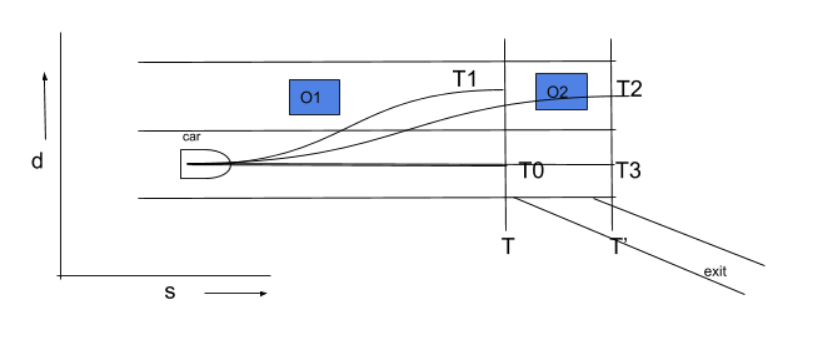
\includegraphics[width=0.8\textwidth]{Images/horizaon_optimality_2.png}
    \caption{Horizon Optimality reference}
    \label{horizon_optimality}
\end{figure}
 
 \todo{move to future works}
 Another horizon generally in the discussion for a planner is spatial horizon which discusses how long is the path generated, as per this planning criteria at low velocities the spatial horizon considered is very small thus the planner may not make right decisions because of conditions like missing the obstacles ahead etc. This shortcoming can be improved by creating a spatial path with the longer horizon in the behavioural layer at lower speeds and allowing the local planner to follow new spatial path than following the global reference path. This is an efficient method as the path planning is less expensive than trajectory planning. As shown in figure \ref{optimized_reference}, following the original reference path(solid line) will lead to trajectories that turn a lot causing discomfort due to obstacles on the side of the road that enter the road, thus by using an optimized reference path(dotted line), ego vehicle can plan efficiently even using short horizons.

The resolution of the sampling in acceleration selection and lateral distance selection will also affect the optimality of planning, a chosen plan can only be optimal of the trajectories created by sampling, higher the number of samples, larger are the possibilities, and the best selection is possible. 

From the above discussion, it can be stated that a planner that has a longer spatial horizon for path planning and short time horizons for trajectory planning will lead to an efficient planner. 
 
 \begin{figure}[h]
    \centering
    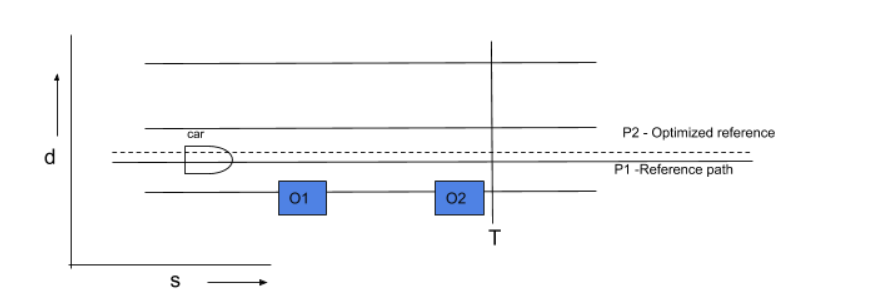
\includegraphics[width=0.8\textwidth]{Images/optimized_reference.png}
    \caption{Optimized Reference Path}
    \label{optimized_reference}
\end{figure}

\subsection{Feasibility}
\label{feasibility}
The ability of the vehicle to traverse the created trajectory determines feasibility. Generally, the curvature of the path, smoothness and accelerations determine whether a trajectory is feasible or not. The proposed planner creates feasible trajectories at lower speeds because of the third order splines used, and higher speeds require fifth or higher order splines to maintain continuity in path and speed. Discussions in \cite{cmu_parallel_thesis} \cite{ppt_teqniqs_coll_Avdnce} throw light on how to achieve higher degrees of smoothness, which approach is better in which driving conditions. As the intended application for this thesis is a modelcar, constant acceleration profiles are used due to a limitation in the ability of the car to track small changes in velocity and inaccuracies in measurement. These can be easily replaced by a smoother higher order polynomial with a better hardware platform. Consistency in paths evaluated with respect to previous plan is another factor in testing feasibility, the current planner penalizes trajectories deviating from previous plan and also take into account current orientation of the vehicle in choosing a path. Thus creating smoother transitions from one state to another by respecting current driving orientation. 

\subsection{Completeness}
\label{completeness}
An algorithm is said to be complete if it can result in a solution every time. A motion planner can be called complete if it returns path if it exists in the space searched. Like many other sampling-based approaches the planner proposed in this thesis only probabilistically complete. That is, the probability of finding a solution approaches to one as the number of samples increases. If there are a higher number of samples in the configuration space, the higher are the chances of finding a solution. If a planner cannot find a solution within the sampled region it forces the car to go into the emergency manoeuvre. 

In Figure \ref{probablistically_complete}, there are only two sampled end states and there is no solution found by the vehicle, by increasing the number of lateral samples a solution can be easily found. In general condition of completeness can be improved in two ways, first is to sample as many points as possible and as closely as possible in the solution space. The second method is to keep on sampling till an end solution is found or timeout has been reached. The former method will reduce the computational performance while the later can be complex and expensive also. The planner proposed in this thesis implements a combination of both methods, as many samples as possible but evaluates only till a feasible solution is found. It is recommended to achieve completeness for safety purposes in autonomous driving. 

 \begin{figure}[h]
    \centering
    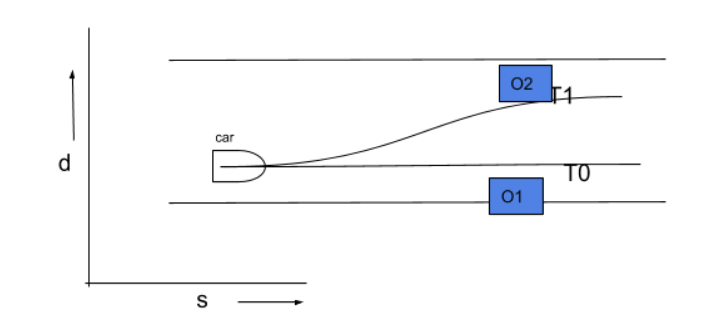
\includegraphics[width=0.8\textwidth]{Images/probablistically_complete.png}
    \caption{Probablistic Completeness}
    \label{probablistically_complete}
\end{figure}

\subsection{Runtime}

Though computation power is available cheaply, it is important to create solutions which are cheaper and can be employed in large scale. In this case, sampling based approaches perform well and run on low computational hardware. In contrast lattice-based approaches such as \cite{cmu_parallel_thesis} \cite{diss_shui_phd_thesis} \cite{werling_frenet} computationally expensive and require a GPU to run. Low computational costs mean larger chances to be adopted to a greater number of platforms.

To compute the complexity of planner lets consider $n_a$ denote the number of acceleration/deceleration profiles, $n_s$ denote the stopping deceleration profiles and $n_l$ denote the number of lateral distance samples. Then the maximum number of samples created is $(n_a+n_s)*n_l$, generally stopping profiles are less as at higher deceleration lower number of lateral samples are chosen due to limitations in vehicle dynamics. This thesis employs a hybrid combination of two methods mentioned in \ref{completeness} to achieve completeness. Therefore in the best case, only one trajectory is evaluated, and complexity is $O(1)$, and the worst case complexity is $O((n_a+n_s)*n_l)$.

Trajectory evaluation with respect to dynamic obstacles is an expensive process in the evaluation of trajectories. Simulation-based methods as discussed in  \cite{kolski_thesis} are expensive with complexity in terms of $O(n_o*n_n)$ where $n_o$ is the number of obstacles and $n_n$ is the number of simulation steps. This thesis employs a simple collision checking algorithm with constant time for evaluating one obstacle thus reducing the complexity to $O(n_o)$, number of obstacles. This process is not effective in intersections. Currently, a conservative approach to wait for other obstacles to pass is used, a simple approach as discussed in \cite{rrt_star} which has a performance better than the simulation-based algorithms can also be employed in future.  

\todo{Write about the execution time for different number of samples, maximum execution time, minimum time from evaluation result etc}

\subsection{Deliberative Approach}
The planner proposed in this thesis maintains a mix of deliberative and reactive approach. Deliberative by evaluating a trajectory completely before committing to it, this is important to create trajectories adhering to traffic, safe and comfortable. In general, all the planners evaluate all the sampled trajectories then choose the best based on different costs. The planner proposed in this thesis does not follow this convention, and once it finds the best trajectory, it stops evaluating the other trajectories as presented in subsection \ref{traj_Selection}. It does not limit the real-time response of the trajectory as the sampling is chosen such that the worst case response time is within the hard real-time response required by the planner. 

%\subsection{Low Computational Costs}

%Though computation power is available cheaply, it is important to create solutions which are cheaper and can be employed in large scale. In this case sampling based approaches generally fare well and run on a low computational hardware. In contrast lattice based approaches such as \cite{cmu_parallel_thesis} \cite{diss_shui_phd_thesis} \cite{werling_frenet} computationally expensive and require a GPU to run. Low computational costs can enable the technology to be adopted to a larger market. Safety should not be compromised for sake of low computational costs and the planner proposed here employs large range of acceleration profiles to bring the vehicle to halt easily in case of an emergency.

%It is true that computation is cheaper in current generation but it is important to bring down the costs to bring technology closer to larger markets. All the lattice based planners which provide the best of the performance evaluate on an average of 100,000 trajectories in one planning cycle and depend on GPUs and many multicore processing units to achieve this results. On the other hand sampling based approaches are cheaper and more conservative. The planner proposed in \cite{cmu_parallel_thesis} can perform a double lane change evasive manoeuvre equivalent to professional drivers to avoid sudden obstacles.  



%\section{Comparisons to other Planners}

\todo{Comparison here doesn't make sense as there are no numbers to compare with other planners, theoretical comparisons can be presented in related work in forms of short comings in different planners. Here may be just add a table like in CMU or DISS shui thesis with comparision to other planner}

%All the motion planners proposed achieve similar objective of navigating smoothly on road with different special capability, these special techniques define how and where these planners can be used. It is tough to compare the planners performance by comparing in definite scenarios due to logistical constraints and costs and objectives of different planners. The generic parameters which define the performance of a trajectory planner are deliberative evaluation, higher dimensional search space, on-road, parallel, real-time. Different types of planners proposed achieve different goals and are suitable at different conditions. 

%\subsection{Comparison to Sampling based Approaches}
%There have been many sampling based approaches that are proposed as discussed in Section \ref{related_work} for trajectory planning. One of such approach is discussed in \cite{traj_smoothing}, here the authors differentiate between the path planning and velocity planning, this approach doesn't choose a spatial or temporal horizon before thus, at high speeds it may fall short if the sampled position is shorter and at low speeds the planned path is very far into the future such that the plan is not valid anyway after some time. This un-necessarily increases the complexity. 

%\subsection{Comparison to Lattice based approaches}
%As discussed in Section \ref{related_work}, lattice based approaches are expensive computationally(generally in terms of fourth order or more based on number of dimensions in lattice), they employ lesser number of acceleration profiles as discussed in \cite{cmu_parallel_thesis} \cite{diss_shui_phd_thesis} to reduce the complexity, this could be a real problem in driving in traffic scenarios where vehicles are close to each other with not so much space for evasive manoeuvres and hard breaking is needed. Though the planner proposed in this thesis cannot create single trajectory with multiple lateral shifts to perform evasive manoeuvres like any other sampling based approach proposed, this planner employs large number of accelerations and deceleration's to improve safety. These planners are designed to run on a separate hardware such as GPU and are not suitable for low computational platforms such as modelcar. 



%Advantages of combining path and velocity? - How it can reduce sampling state. 

%Acceleration profiles for emergency stopping 

%Simulation based approaches to the proposed approach in this planner for collision checking. 

%Why it is not important to validate other trajectories once the best trajectory is found. 

%Urban driving needs strong abilities to stop immediately and lattice planners cannot do this as the number of acceleration profiles increases the evaluated trajectories gets increased in thousands. 

%Eg: CMU - increasing one acceleration will add 13000+ more trajectories, discretizing time by one more step will add 200,000 thousand more trajectories to evaluate thus limit the spatial and temporal horizon the planner can evaluate. At high speeds a larger spatial horizon is needed but generally temporal horizon remains same at all the speeds thus we chose to plan in a temporal horizon to allow planning at all multiple speeds. 


%Divide the trajectory planning and behaviour layer, with this the complexity of solving the task can be reduced drastically. If the trajectory planner need not worry about the behaviours and focus solely on driving safely it will enhance the performance of the vehicle and achieve the costs at a low computational cost.  



